\documentclass{article}
\usepackage[table]{xcolor}
\usepackage[english]{babel}
\usepackage[letterpaper,top=2cm,bottom=2cm,left=3cm,right=3cm,marginparwidth=1.75cm]{geometry}
% Useful packages
\usepackage{amsmath}
\usepackage{graphicx}
\usepackage[colorlinks=true, allcolors=blue]{hyperref}
\usepackage{caption}
\usepackage[inline]{enumitem}
\title{Deliverable 1 \\}
\author{DEPARTMENT OF COMPUTER SCIENCE AND SOFTWARE ENGINEERING\\\\\\SOEN 6461: SOFTWARE DESIGN AND METHODOLOGIES\\WINTER 2023\\\\\\\textbf{Submitted to:} \textit{Dr. Pankaj Kamthan}\\\\\textbf{By}, \\\textbf{(Team O)}\\\\\\\textit{Bharat Saini(40202642)}\\\textit{Adwait Sambare (40162664)}\\\textit{Sagar Sanghani(40186043)}\\\textit{Santhosh Santhanam (40202625)}\\\textit{Khushboo Saraf (40204421)}}
\date{}

\begin{document}
\maketitle

\begin{center}
\large{URL: \href{}https://github.com/bharat882/SOEN6461{}}
\end{center}

\pagebreak
\tableofcontents
\pagebreak
\listoftables
\pagebreak
\listoffigures
\pagebreak

\section{Problem 1}
iGo is an electronic TVM application for STM that will allow passengers to purchase tickets, passes, and access cards for travel without the need for standing in queues. The STM (Société de transport de Montréal) operates the Montreal metro, a rapid transit system that serves the city of Montreal, Quebec, Canada.  iGo allows the customers/passengers to travel within the city of Montreal using a ticket or an e-pass generated by the ticket vending machine. These electronic passes and tickets are validated at the metro stations. iGo application allows the user to manage their iGo account online, thus making it more convenient. \\
iGo supports various payment gateways and allows the passenger to make payment using debit/credit cards, google pay, apple pay. \\

\textbf{Functionality provided by iGo:} 

\begin{itemize}
\item Sign up/Login for iGo
\item Load funds to your iGo account
\item Operator to update the metro routes
\item Purchase tickets and passes
\item View transaction history
\item View available Balance
\item View bought passes and their validity
\end{itemize} 

 \begin{figure}[h!]
  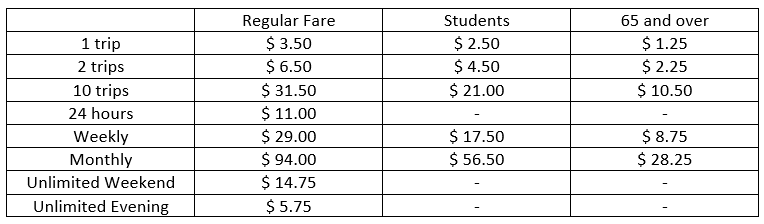
\includegraphics[scale=1.0]{fare.png}
  \caption{STM fare breakdown}
  \label{fig:fare}
\end{figure}

\textbf{Out of Scope:}
\begin{enumerate}
 \item Payment gateway Implementation (One payment option might be provided to mock Adding funds to the card).
 \item Validation of Students/Senior Citizens ID. 
 \item Recovery of account 
 \item Refund of the amount to a bank account 
 \item Validation of time while using various passes.
 \item Bus only passes.
 \item Implementation of Routes. 
\end{enumerate}

\newpage

\section{Problem 2}
The problem domain model here gives how a Ticket Vending Machine is conceptually represented with a software system behind it to solve. It usually captures all the entities, features, and relationships between different processes that exist in the real world. Here the problem domain model for the iGo TVM has the following entities,  
\begin{itemize}
\item Ticket Vending Machine/Kiosk: The main entity in the iGo TVM project. It's an automated, self-service vending machine that produces tickets for public transportation. 
\item Customer/User: A person who uses the TVM to purchase tickets. There are different types of users and for each user, the fare also varies. 
\item Operator: This personnel is like an admin who can add, and delete routes, stations, and fares.
\item Ticket/Pass: This entity represents the ticket that the user receives from the TVM. There are various types of tickets.  
\item Fare: This entity represents the cost of each type of ticket for different customers. The fare breakdown for different customers and ticket types is given in Figure~\ref{fig:fare}. 
\item Payment Transaction: This entity represents the transaction between the TVM and the customer, including the payment. 
\end{itemize}
\subsection{Class diagram}
All the entities above are represented better using a class type. The class diagram has the names, attributes, and relationships between the entities. The classes are as follows, 
\begin{figure}[h!]
    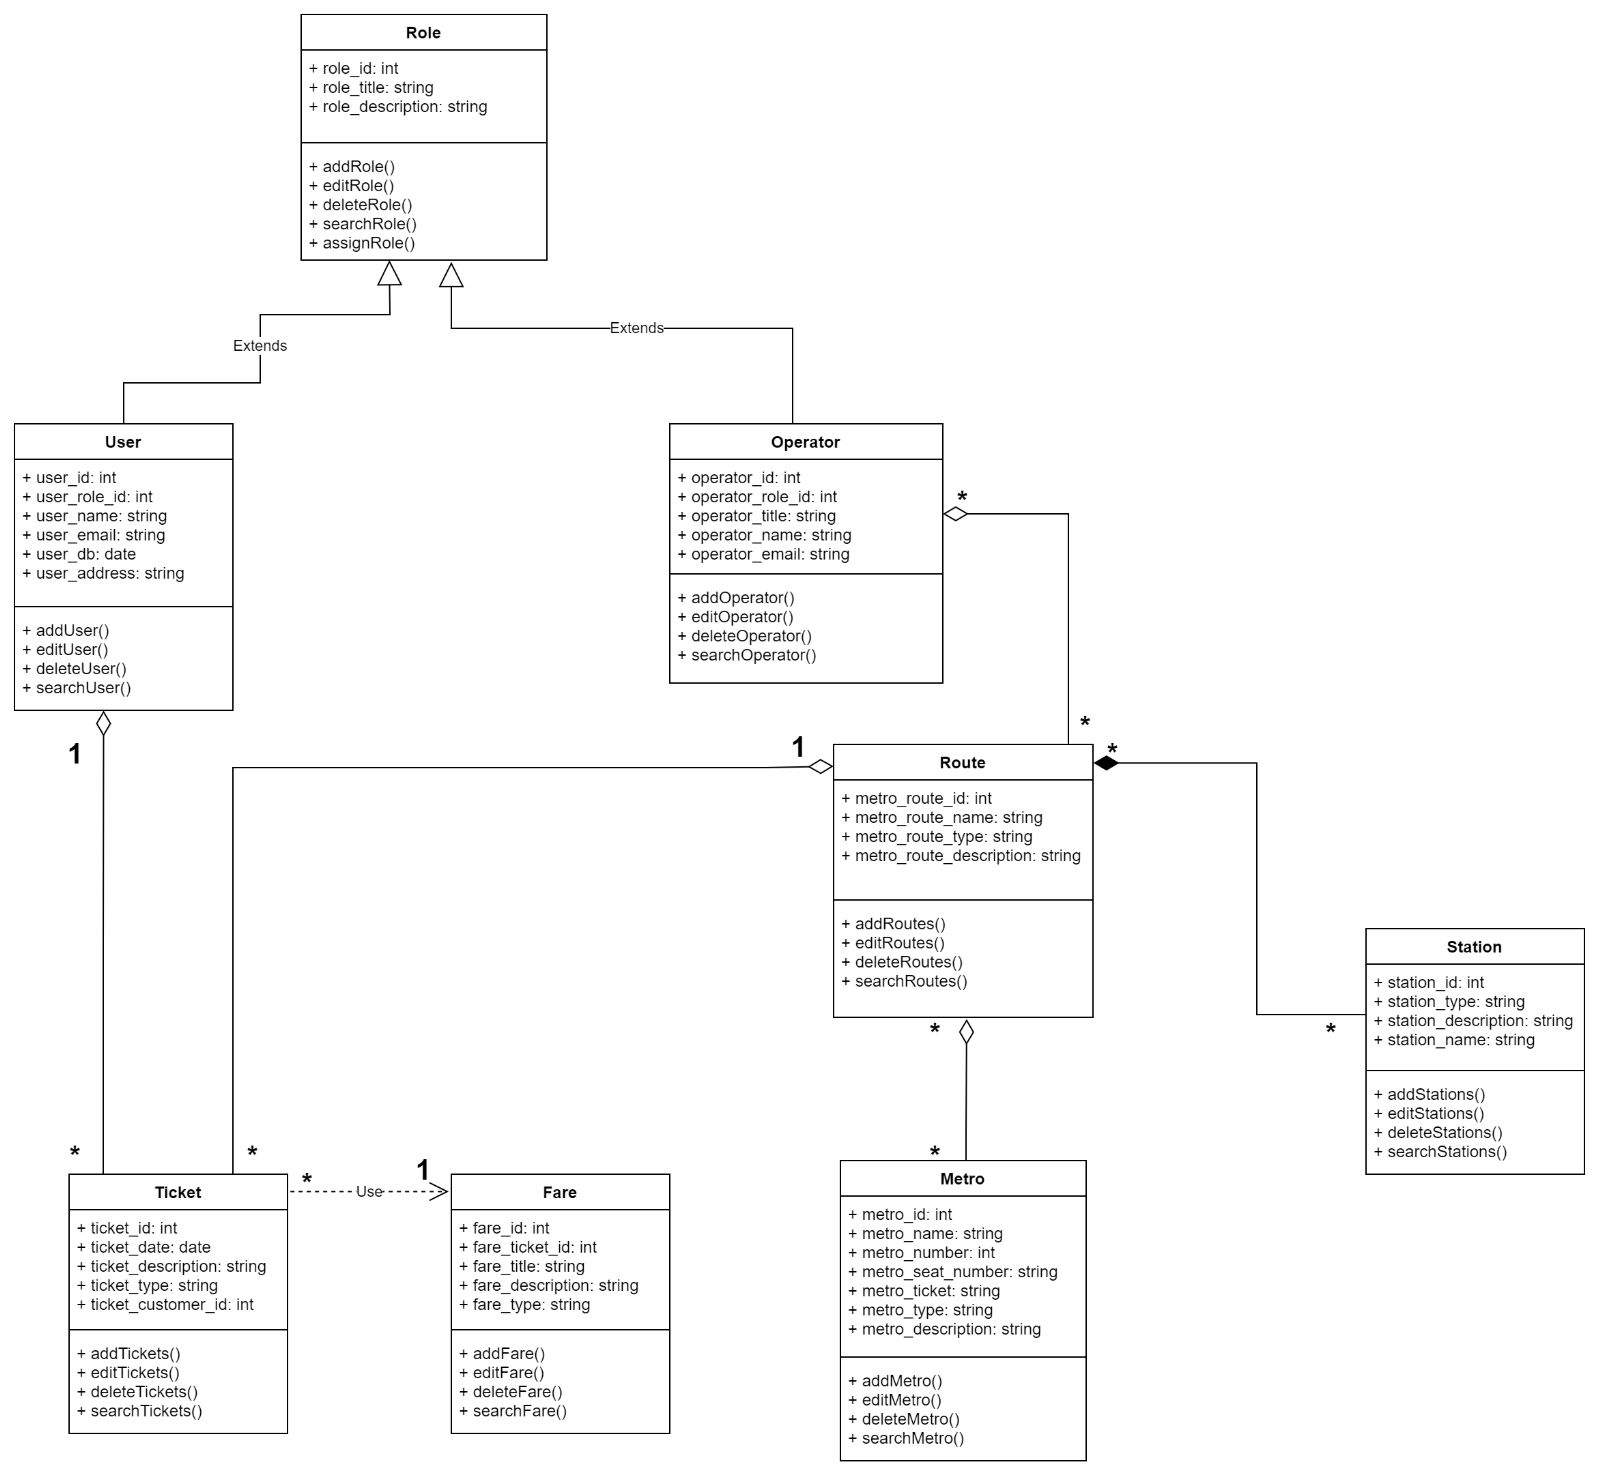
\includegraphics[scale=0.3]{Class diagram.jpeg}
    \caption{Class diagram}
    \label{fig:class}
\end{figure}\
\pagebreak
\subsubsection{Class descriptions}
\begin{itemize}
    \item Role: Role class is used to manage the identity of a person accessing the system. iGo has 2 roles, a user and an operator.
    \item User: User class is used to maintain a database of customers accessing your system. 
    \item Operator: Operator class is used to create operators/admin who maintain the system internally. 
    
    Following are the core services offered by STM which is incorporated in the iGo ticket vending machine. 
    \begin{itemize}
        \item Route: This service is used to add more routes to the internal working model of STM. These routes are accessed and shown to the user to select from and pay the fare for the route selected. 
        \item Stations: This service is used to add, remove, and search stations in a route. So this class has a great relationship and dependency on the route.
        \item Metro: Similar to the stations class we can add, remove and get information on the metro running in a particular route. Also has a great dependency on the route. 
        \item Ticket: This class provides you with the tickets after you choose the route. There are 2 different ticket types. One is the normal ticket for one-time use and the other is a rechargeable, contact-less smart card for fare payment. The User and Fare classes have a strong dependency on Ticket. 
        \item Fare: This class is used to set fares for the route available, based on the ticket type and also on the type of user. Certain age people being children or people aged 65+ have reduced ticket fares in both normal tickets and also in their monthly passes. Students have a reduced fare on their monthly passes. 
    \end{itemize} 
\end{itemize}
\subsubsection{Class relationships}
Relationships between classes define the structure and behavior of the system. Here in iGo, from figure \ref{fig:class} a user has a one-to-many association with the ticket class. A user can have multiple tickets for his journey or tap the card multiple times to and fro a place. The ticket class is associated with a fare such that multiple tickets can have the same fare. Furthermore, the ticket class is associated with the route class in a many-to-one fashion. Station and Metro classes are associated with the Route class in many-many ways as many routes can have many stations and metros associated with them with possible overlaps. Routes are managed by an Operator and multiple operators can manage multiple stations. And finally, the User and Operator extend the Role class which consists of common attributes of a Role.
\subsection{Package diagram}
A package diagram can provide us with a more structural high-level organization of class entities. For iGo, the classes that work together, and extend each other are carefully considered and made into a package.
\begin{figure}
    \centering
    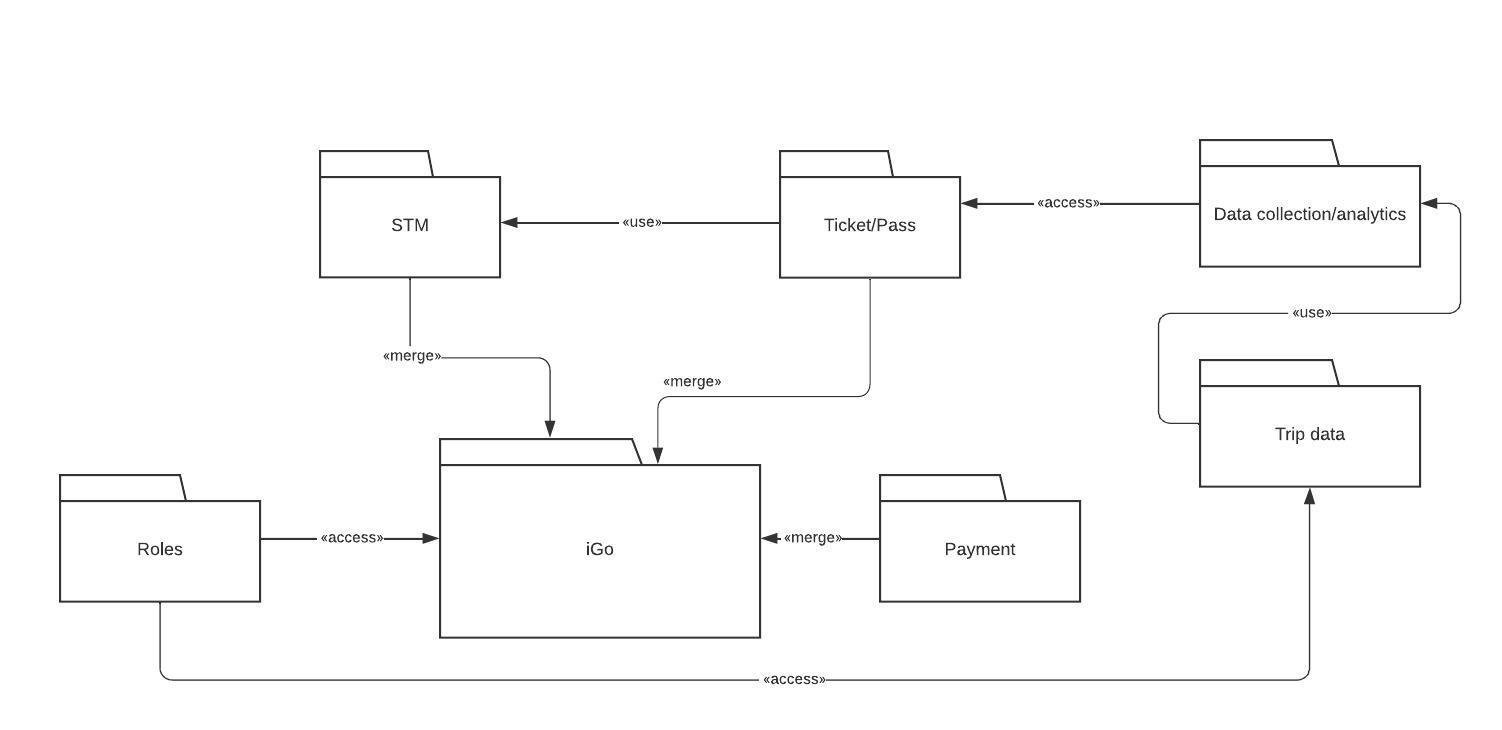
\includegraphics[scale=0.5]{UML package diagram.jpeg}
    \caption{Package diagram}
    \label{fig:package}
\end{figure}

\subsubsection{Package descriptions}
\begin{itemize}
    \item Roles: Not all the classes and functionalities can be accessed by everyone. The User and Operator classes are combined together in this package and access is given according to the type of person.
    \item iGo, the Ticket Vending Machine: This is the main package. All other packages finally merge their functionalities with iGo. 
    \item STM: The STM package contains the working of core services provided by STM. The operator can access the core services of iGo, 
    \begin{itemize}
        \item Routes
        \item Fare
        \item Metro
        \item Stations
    \end{itemize}
    \item Ticket/Pass: The package contains the ticket class which is extended by the fare class used in STM. 
    \item Data Collection/Analytic: The package has classes that access classes from the tickets package and provide the customer with trip data. The following trip data are shown to the user, 
    \begin{itemize}
        \item Transaction history
        \item Get receipts
    \end{itemize}
    \item Payment: This package overall contains the classes required to initiate, and process the payment with the bank using a debit/credit card. 
\end{itemize}
\subsection{Component diagram}
With various modules in the system of iGo, how well these modules interact with one another to complete the system is given by a component diagram. The component diagram gives an end-to-end flow of the system.
\begin{figure}[h]
    \centering
    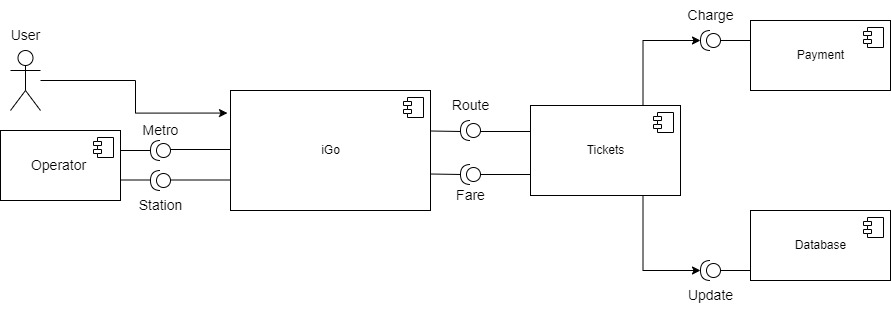
\includegraphics[scale=0.5]{component diagram.jpg}
    \caption{Component diagram}
    \label{fig:component}
\end{figure}
\pagebreak
All the operations that a component uses to interact with the other component are represented with a circle on top of the relationship. An Operator can add metro, stations to the iGo system. The user accessing the iGo system gets his tickets based on the route and fare he chooses. The tickets are in turn charged by the credit card company and the database is updated for the user to view his transactions later. 
\pagebreak
\section{Problem 3}
\subsection{Mind map for Interview process}
Interviews can actually be a valuable tool for developing software. They are used to gather information from different people using the system, knowing the expectations from people, etc. After the problem domain model has been developed, the interview process helps validate and test them in the real world. These help us identify the inconsistencies in our model. 
Similarly, for our project iGo we have set up an interview process. For the interview process, a mind map is created to decide the necessary elements needed for the interview process. Mind maps are generally used to have a more organized, focused, and efficient way of interviewing. The mind map also facilitates better communication and understanding between interviewers and interviewees. 
Following is the mind map created for iGo, 
\begin{figure}[h]
    \centering
    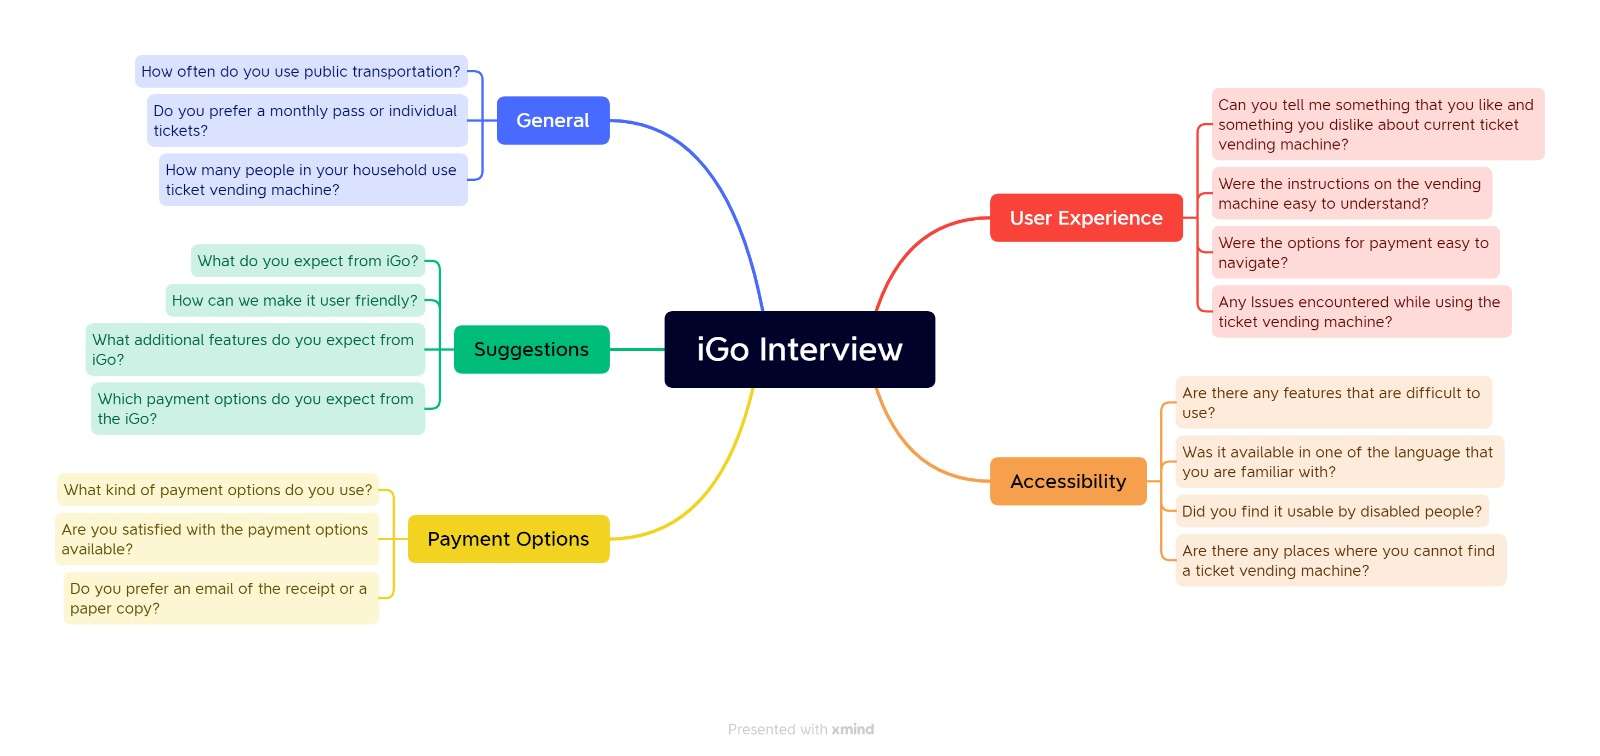
\includegraphics[scale=0.3]{Mind map.jpeg}
    \caption{Mind map}
    \label{fig:map}
\end{figure}

The mind map has various categories branching out namely, general questions about the system, suggestions to improve the design, feedback on the user experience, how easy it is to access the system, and about the payment options. For the interview transcripts please refer to the \nameref{Appendix} section. 

\subsection{Conclusion}
From the interviews, it was evident that the majority of interviewees were willing to use an online application to purchase tickets or monthly passes. It was revealed that the current ticket vending machine is highly reliable and it almost never fails. There was a high number of unique suggestions for additional features of the iGo, and some of these correlated with the features we decided to include.
\pagebreak
 \section{Problem 4}
 Now for the system, we need to know how these elements are physically related to one another. This gives us an idea for organizing, grouping, and visual representation of which stakeholder is going to use which element, etc. This gives a very clear understanding of the system's design and implementation between developers, designers, and stakeholders. 
 \subsection{Use case diagram}
 \begin{figure}[h]
    \centering
    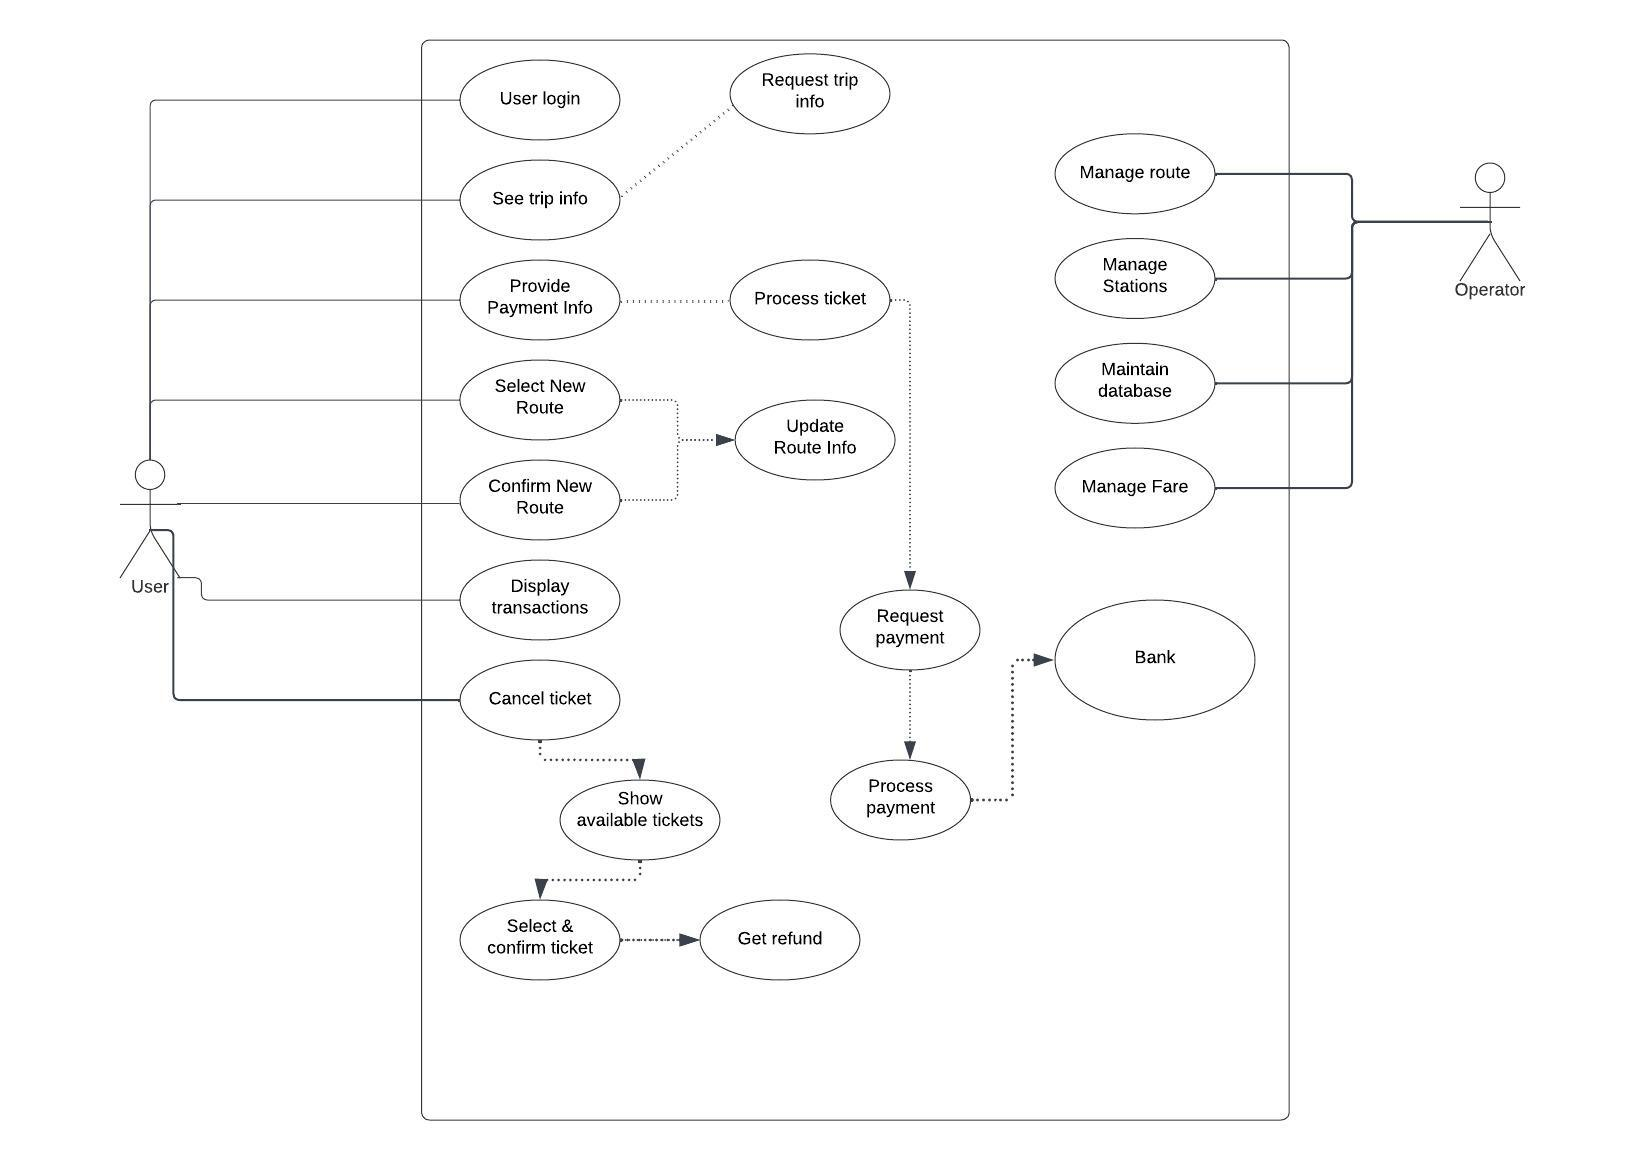
\includegraphics[scale=0.7]{use case.jpeg}
    \caption{Use case diagram}
    \label{fig:useCase}
\end{figure}
\pagebreak
\subsubsection{Use case descriptions}
\begin{table}[ht]
    \centering
    \begin{tabular}{|l|p{11cm}|}
         \hline
         System& iGo\\
         \hline
         Use case no. & 1 \\
         \hline
         Name & User login \\
         \hline
         Pre-Condition(s)   & 
         \begin{enumerate*}[itemjoin=\newline]
             \item User at the ticket vending machine
         \end{enumerate*} \\
         \hline
         Post-Condition(s)  & 
         \begin{enumerate*}[itemjoin=\newline]
             \item User gets his ticket 
         \end{enumerate*} \\
         \hline
         Trigger& User places the card for recharging or clicks on the new ticket option \\
         \hline
         Normal Flow        & 
         \begin{enumerate*}[itemjoin=\newline]
             \item When he taps his e-pass it shows the services offered i.e. routes, fare, and payment. 
         \end{enumerate*} \\
         \hline
         Exceptional Flow(s)& None\\
         \hline
         Related Actor(s)   & User/Passenger\\
         \hline
         Related Use Case(s)& None\\
         \hline
    \end{tabular}
    \caption{User login}
    \label{tab:UC_login}
\end{table}
\begin{table}[ht]
    \centering
    \begin{tabular}{|l|p{11cm}|}
         \hline
         System& iGo\\
         \hline
         Use case no. & 2 \\
         \hline
         Name & See Trip Info \\
         \hline
         Pre-Condition(s)   & 
         \begin{enumerate*}[itemjoin=\newline]
             \item User logged in to the system
         \end{enumerate*} \\
         \hline
         Post-Condition(s)  & 
         \begin{enumerate*}[itemjoin=\newline]
             \item Receives various services offered
         \end{enumerate*} \\
         \hline
         Trigger& User clicks on the request trip info column from the ticket vending machine \\
         \hline
         Normal Flow        & 
         \begin{enumerate*}[itemjoin=\newline]
             \item The trip info from the STM is fetched and returned to the user in the ticket vending machine.  
         \end{enumerate*} \\
         \hline
         Exceptional Flow(s)& None\\
         \hline
         Related Actor(s)   & User/Passenger\\
         \hline
         Related Use Case(s)& Request Trip Info\\
         \hline
    \end{tabular}
    \caption{See trip info}
    \label{tab:UC_tripInfo}
\end{table}
\pagebreak
\begin{table}[ht]
    \centering
    \begin{tabular}{|l|p{11cm}|}
         \hline
         System& iGo\\
         \hline
         Use case no. & 3 \\
         \hline
         Name & Provide payment info \\
         \hline
         Pre-Condition(s)   & 
         \begin{enumerate*}[itemjoin=\newline]
             \item User logged in to the system and has chosen a route 
         \end{enumerate*} \\
         \hline
         Post-Condition(s)  & 
         \begin{enumerate*}[itemjoin=\newline]
             \item Receives various services offered
         \end{enumerate*} \\
         \hline
         Trigger& User click on the payment option \\
         \hline
         Normal Flow        & 
         \begin{enumerate*}[itemjoin=\newline]
             \item TVM asks the commuter to provide the card details or insert the card in the machine.   
         \end{enumerate*} \\
         \hline
         Exceptional Flow(s)& None\\
         \hline
         Related Actor(s)   & User/Passenger\\
         \hline
         Related Use Case(s)& None\\
         \hline
    \end{tabular}
    \caption{Payment info}
    \label{tab:UC_paymentInfo}
\end{table}
\begin{table}[ht]
    \centering
    \begin{tabular}{|l|p{11cm}|}
         \hline
         System& iGo\\
         \hline
         Use case no. & 4 \\
         \hline
         Name & Update Route Info \\
         \hline
         Pre-Condition(s)   & 
         \begin{enumerate*}[itemjoin=\newline]
             \item User logged in to the system and has booked a ticket 
         \end{enumerate*} \\
         \hline
         Post-Condition(s)  & 
         \begin{enumerate*}[itemjoin=\newline]
             \item His route info for the ticket selected in updated
         \end{enumerate*} \\
         \hline
         Trigger& User click on the update route option \\
         \hline
         Normal Flow        & 
         \begin{enumerate*}[itemjoin=\newline]
             \item iGo asks the commuter to select a new route and confirm it. This gives an updated route ticket.    
         \end{enumerate*} \\
         \hline
         Exceptional Flow(s)& None\\
         \hline
         Related Actor(s)   & User/Passenger\\
         \hline
         Related Use Case(s)& Select New Route and Confirm Route\\
         \hline
    \end{tabular}
    \caption{Update route info}
    \label{tab:UC_updateRoute}
\end{table}
\begin{table}[ht]
    \centering
    \begin{tabular}{|l|p{11cm}|}
         \hline
         System& iGo\\
         \hline
         Use case no. & 5 \\
         \hline
         Name & Display Transactions \\
         \hline
         Pre-Condition(s)   & 
         \begin{enumerate*}[itemjoin=\newline]
             \item User logged in to the system
         \end{enumerate*} \\
         \hline
         Post-Condition(s)  & 
         \begin{enumerate*}[itemjoin=\newline]
             \item All the previous transactions made are shown
         \end{enumerate*} \\
         \hline
         Trigger& User click on the view transactions option \\
         \hline
         Normal Flow        & 
         \begin{enumerate*}[itemjoin=\newline]
             \item iGo provides previous transactions with the card company and also gives various options to filter from   
         \end{enumerate*} \\
         \hline
         Exceptional Flow(s)& None\\
         \hline
         Related Actor(s)   & User/Passenger\\
         \hline
         Related Use Case(s)& None\\
         \hline
    \end{tabular}
    \caption{Display transactions}
    \label{tab:UC_transactions}
\end{table}
\begin{table}[ht]
    \centering
    \begin{tabular}{|l|p{11cm}|}
         \hline
         System& iGo\\
         \hline
         Use case no. & 6 \\
         \hline
         Name & Cancel ticket \\
         \hline
         Pre-Condition(s)   & 
         \begin{enumerate*}[itemjoin=\newline]
             \item User logged in to the system
         \end{enumerate*} \\
         \hline
         Post-Condition(s)  & 
         \begin{enumerate*}[itemjoin=\newline]
             \item Ticket has been canceled successfully and the money is refunded.
         \end{enumerate*} \\
         \hline
         Trigger& User click on the cancel ticket option \\
         \hline
         Normal Flow        & 
         \begin{enumerate*}[itemjoin=\newline]
             \item iGo shows the available tickets to choose from. 
             \item User chooses and confirms the tickets to be canceled. 
             \item The money is refunded to the account. 
         \end{enumerate*} \\
         \hline
         Exceptional Flow(s)& None\\
         \hline
         Related Actor(s)   & User/Passenger\\
         \hline
         Related Use Case(s)& None\\
         \hline
    \end{tabular}
    \caption{Cancel ticket}
    \label{tab:UC_cancel}
\end{table}
\begin{table}[ht]
    \centering
    \begin{tabular}{|l|p{11cm}|}
         \hline
         System& iGo\\
         \hline
         Use case no. & 7 \\
         \hline
         Name & Manage routes \\
         \hline
         Pre-Condition(s)   & 
         \begin{enumerate*}[itemjoin=\newline]
             \item Operator successfully logged in to the system
         \end{enumerate*} \\
         \hline
         Post-Condition(s)  & 
         \begin{enumerate*}[itemjoin=\newline]
             \item Add, delete or update any new routes information
         \end{enumerate*} \\
         \hline
         Exceptional Flow(s)& None\\
         \hline
         Related Actor(s)   & Operator\\
         \hline
         Related Use Case(s)& None\\
         \hline
    \end{tabular}
    \caption{Manage Routes}
    \label{tab:UC_route}
\end{table}
\pagebreak
\begin{table}[ht]
    \centering
    \begin{tabular}{|l|p{11cm}|}
         \hline
         System& iGo\\
         \hline
         Use case no. & 8 \\
         \hline
         Name & Manage stations \\
         \hline
         Pre-Condition(s)   & 
         \begin{enumerate*}[itemjoin=\newline]
             \item Operator successfully logged in to the system
         \end{enumerate*} \\
         \hline
         Post-Condition(s)  & 
         \begin{enumerate*}[itemjoin=\newline]
             \item Add, delete or update any new station information
         \end{enumerate*} \\
         \hline
         Exceptional Flow(s)& None\\
         \hline
         Related Actor(s)   & Operator\\
         \hline
         Related Use Case(s)& None\\
         \hline
    \end{tabular}
    \caption{Manage Station}
    \label{tab:UC_station}
\end{table}
\begin{table}[ht]
    \centering
    \begin{tabular}{|l|p{11cm}|}
         \hline
         System& iGo\\
         \hline
         Use case no. & 9 \\
         \hline
         Name & Manage fare \\
         \hline
         Pre-Condition(s)   & 
         \begin{enumerate*}[itemjoin=\newline]
             \item Operator successfully logged in to the system
         \end{enumerate*} \\
         \hline
         Post-Condition(s)  & 
         \begin{enumerate*}[itemjoin=\newline]
             \item Add, delete or update any  fare information
         \end{enumerate*} \\
         \hline
         Exceptional Flow(s)& None\\
         \hline
         Related Actor(s)   & Operator\\
         \hline
         Related Use Case(s)& None\\
         \hline
    \end{tabular}
    \caption{Manage Fare}
    \label{tab:UC_fare}
\end{table}
\pagebreak
From figure \ref{fig:useCase} all the dotted lines represent the dependency that a particular use case has on the other. It means that the use cases are related to one another.  
\pagebreak
 \section{Problem 5}
 \subsection{Activity diagram}
 After the problem domain modeling is created, interviews are completed, and also knowing the different use cases that are considered, we can now model the behavior of the system over time. These temporal relationships help us define the sequence of events that occur in the system. Temporal relationships also give us an idea of how use cases interact with each other. 
 \subsubsection{Commuter booking a ticket}
     \begin{figure}[h]
        \centering
        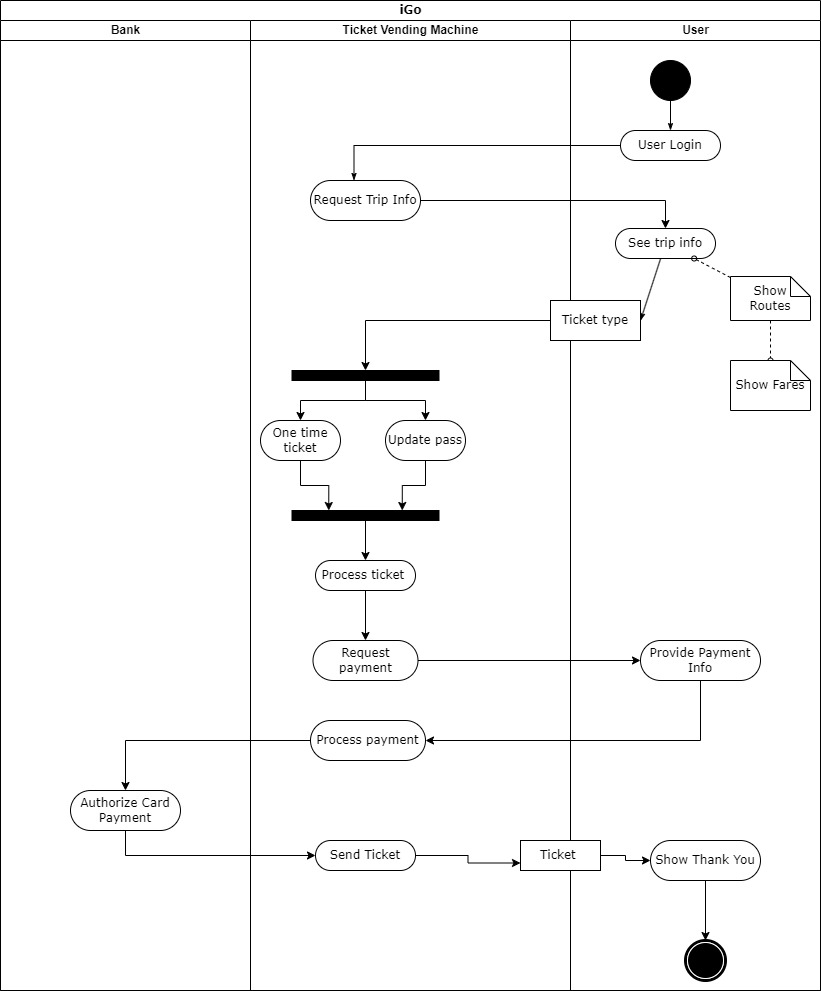
\includegraphics[scale=0.3]{booking_ticket.jpg}
        \caption{Commuter booking a ticket}
        \label{fig:booking}
    \end{figure}
    This activity shows the use cases involved when a user is booking a ticket using the iGo ticket vending machine. It starts with the user logging in to the system. The iGo TVM shows all the trip info like the route to select and the fare shown beside it. The user selects a particular route and the ticket is processed. For the ticket's fare payment the user is asked to provide the payment details and the payment is authorized by the bank. 
    \pagebreak
 \subsubsection{Commuter updating/canceling a ticket}
     \begin{figure}[h]
        \centering
        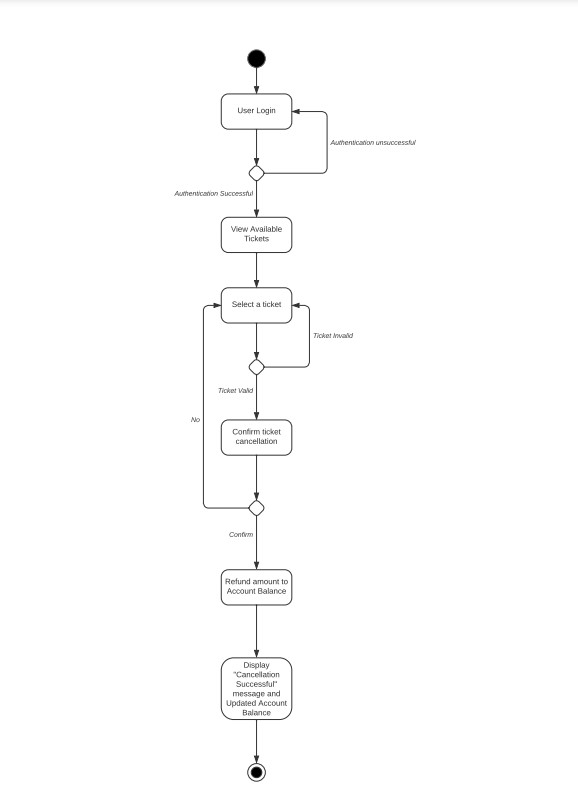
\includegraphics[scale=0.5]{update_ticket.jpg}
        \caption{Commuter updating/canceling a ticket}
        \label{fig:updateTicket}
    \end{figure}
    This activity shows the use cases involved in updating/canceling a ticket. The user logs in and views his available tickets. From the tickets that are booked, he has to select the one that he wants to cancel. The tickets are canceled after confirmation and the fare paid is returned back to the user. 
 \subsubsection{Operator adding stations/routes}
     \begin{figure}[h]
        \centering
        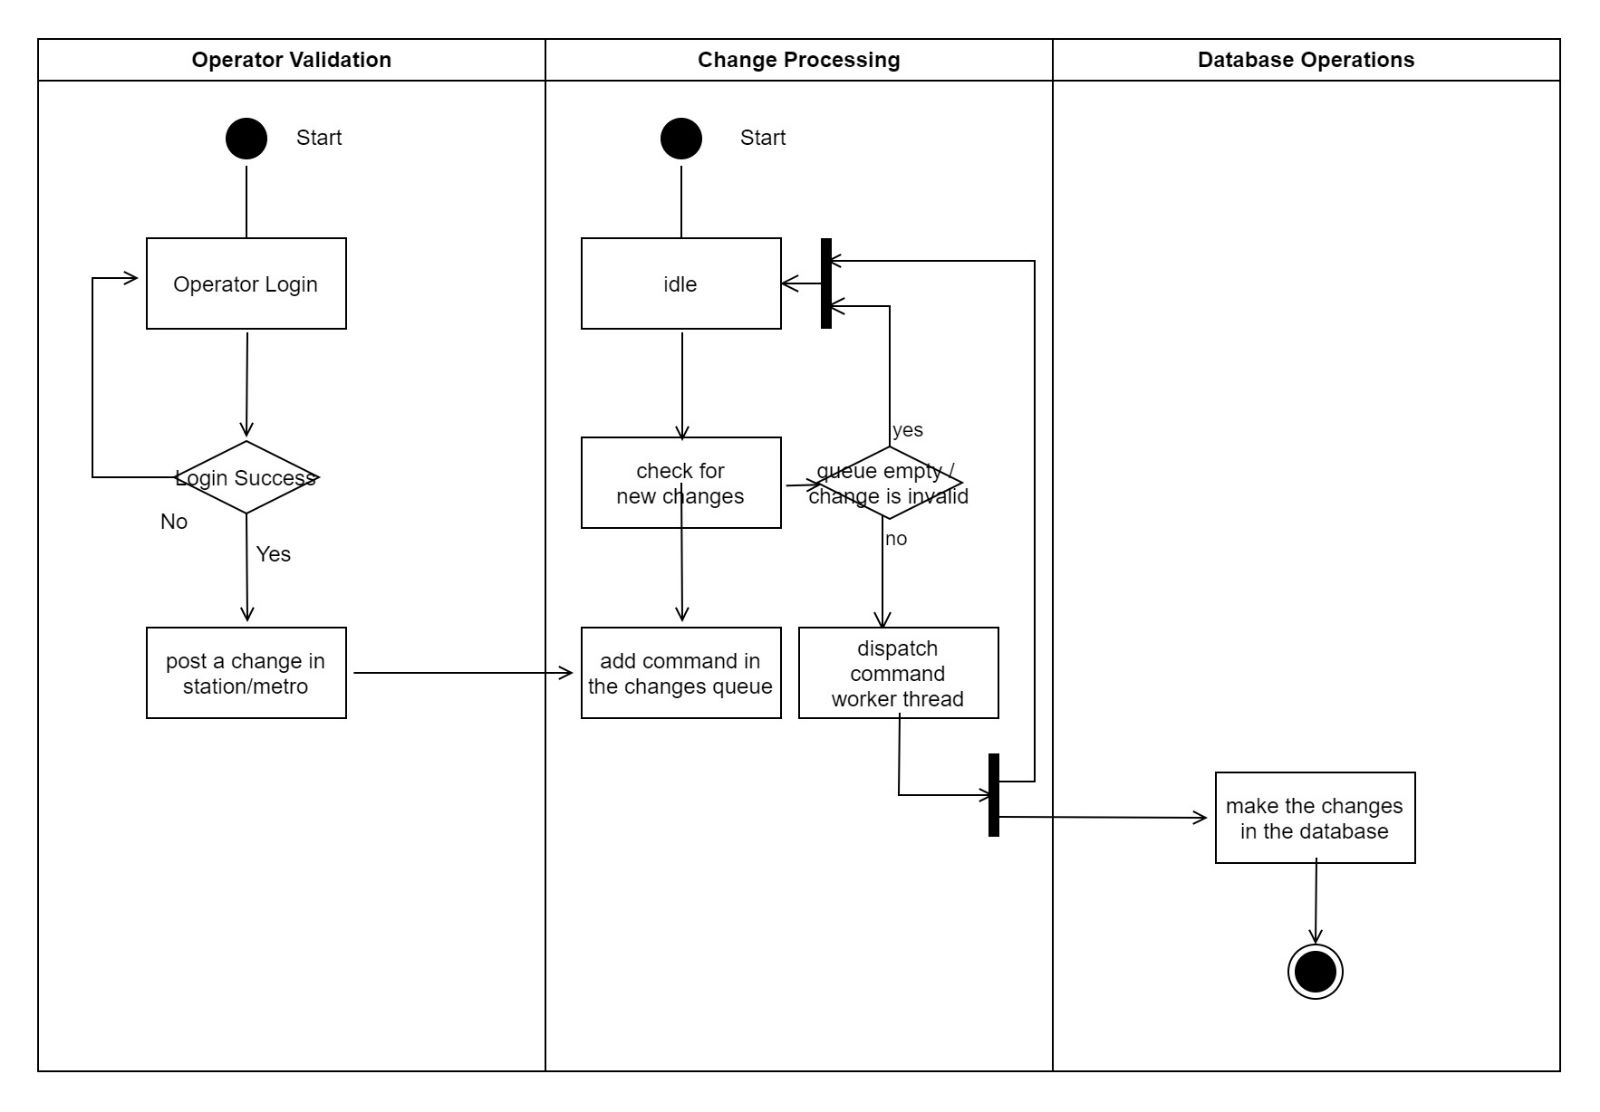
\includegraphics[scale=0.2]{operator.jpeg}
        \caption{Operator adding stations/routes}
        \label{fig:operator}
    \end{figure}
    This activity shows how an operator can change routes, fares, etc in the database. At first, the operator is validated and he initiates the change in the core services accessible. The initiated changes are added to a queue and are handled one by one using a worker thread. Finally, these threads make the changes in the database. 
 \subsubsection{Commuter changing routes/schedules}
     \begin{figure}[h]
        \centering
        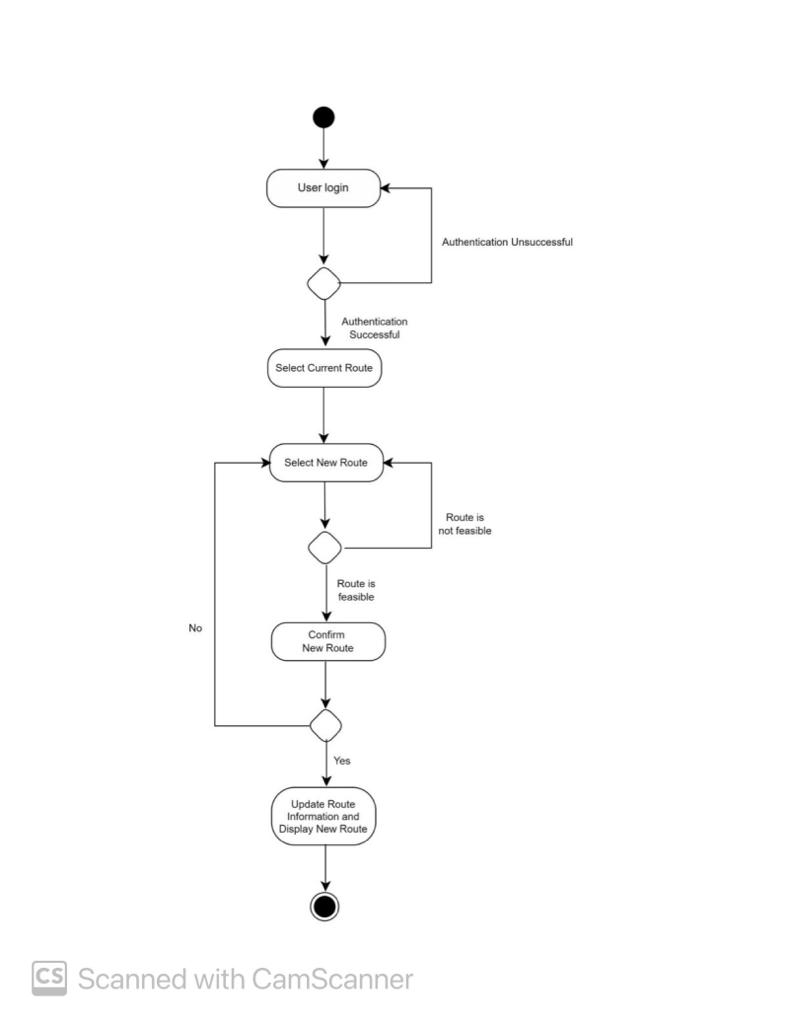
\includegraphics[scale=0.4]{customer_changing_route.jpeg}
        \caption{Commuter changing routes/schedules}
        \label{fig:route}
    \end{figure}
    This activity allows the user to change the route for the same ticket or changes to the schedule. The User logs in and selects the current route he wants to change. Then the user has to select a new route and the TVM validates whether the updated route is feasible or not and the changes are done to the ticket.  
    \pagebreak
 \subsubsection{Commuter views transaction history}
    \begin{figure}[h]
        \centering
        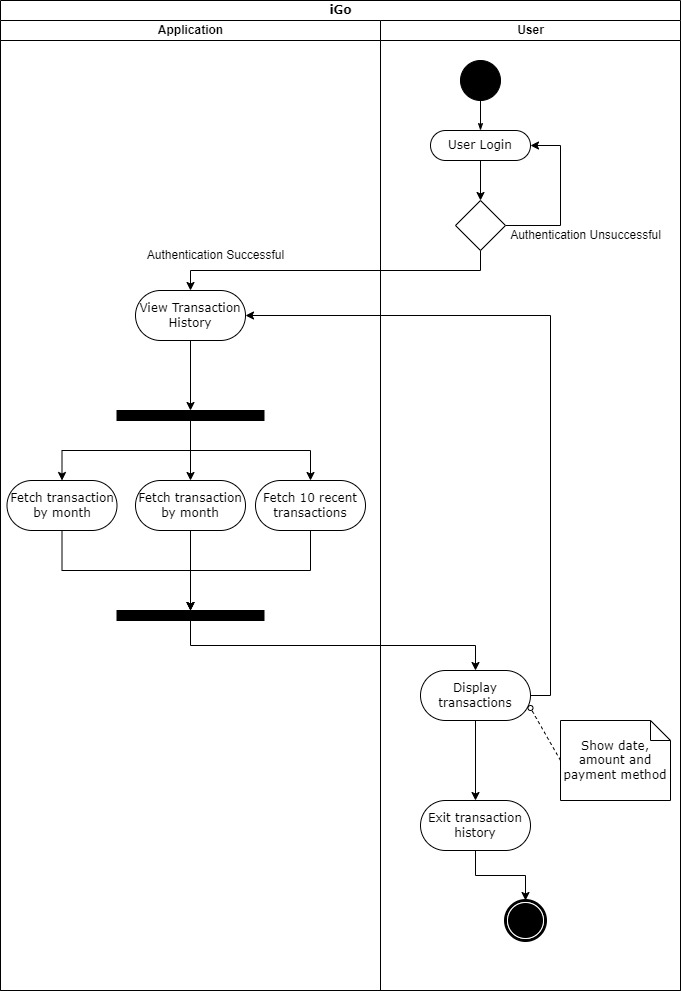
\includegraphics[scale=0.25]{transaction_history_activity.jpg}
        \caption{Transaction history}
        \label{fig:history}
    \end{figure}
    This activity allows the user to view his transaction history. The user logs in and after successful authentication, the user is given 3 options namely, transaction by month, transaction by year, or his recent 10 transactions. The transaction shows the date, fare, and payment method used. The user can also get the receipts generated online. 
\pagebreak
 \section{Appendix} \label{Appendix}
 \subsection{Interview Transcripts}
 \subsubsection{Interview 1}The first interview transcript with Interviewer Sagar Sanghani and Interviewee Smit Parmar

\begin{itemize}
    \item[] Sagar Sanghani – Hi, Good Morning. I am working on a project regarding a ticket vending machine for public transportation. Can you spare a few minutes to answer a few questions regarding the same?
    \item[] Smit Parmar – Sure, Go ahead.
    \item[] Sagar Sanghani – Are you a student or a working professional?
    \item[] Smit Parmar – No, I am a student at Concordia University. 
    \item[] Sagar Sanghani – Do you use the public transport system?
    \item[] Smit Parmar – Yes, I use it every day for my commute to the university. I also use it to get around the city, it’s really efficient.
    \item[] Sagar Sanghani – So, tell me something you like and something you dislike about the ticket vending machine.
    \item[] Smit Parmar – I like the ticket vending machine because it is reliable. But I really dislike long queues to get a ticket or recharge my monthly pass.
    \item[] Sagar Sanghani – Okay. Was the ticket vending machine available in one of the languages that you were familiar with?
    \item[] Smit Parmar – Yes, it was available in English and French.
    \item[] Sagar Sanghani – Would you be interested in using an online application to purchase the ticket or buying a monthly pass?
    \item[] Smit Parmar – Yes, it would help.
    \item[] Sagar Sanghani – What additional features can you suggest for the application?
    \item[] Smit Parmar – I would like to have real-time updates on the location and timing of metro and buses
    \item[] Sagar Sanghani – What kind of payment options are you comfortable using online transactions?
    \item[] Smit Parmar – I can use a credit card and a debit card.
    \item[] Sagar Sanghani – Thank you so much for answering these questions. I appreciate your time. Have a good day!
\end{itemize}
\pagebreak


 \subsubsection{Interview 2}The second interview transcript with Interviewer Adwait Sambare and Interviewee Ganesh Viswanathan

\begin{itemize}
    \item[] Adwait Sambare – Hello. I am working on an application for a ticket vending machine. Would you mind answering a few questions? It will take only a few minutes.
    \item[] Ganesh Viswanathan – Okay sure!
    \item[] Adwait Sambare – What do you do in Montreal?
    \item[] Ganesh Viswanathan – I work at a Pharmaceutical Company in Montreal. 
    \item[] Adwait Sambare – Do you use the public transport system or use your own vehicle?
    \item[] Ganesh Viswanathan – I use both.
    \item[] Adwait Sambare – How often do you use the public transport system?
    \item[] Ganesh Viswanathan – I use it once or twice a week.
    \item[] Adwait Sambare – How is your experience with using ticket vending machines for buying tickets? 
    \item[] Ganesh Viswanathan – I think waiting in long queues is the biggest issue for me. That and an old-style display to buy tickets. It is a little confusing for someone using it for the first time.
    \item[] Adwait Sambare – Did you find instructions for payment easy?
    \item[] Ganesh Viswanathan – Not really, the screen to complete the payment using a card is small and dim.
    \item[] Adwait Sambare – Would you prefer buying tickets online from your mobile phone or your PC?
    \item[] Ganesh Viswanathan – Yes, I would, it will save a lot of time.
    \item[] Adwait Sambare – What kind of payment options would you like to use in the online application?
    \item[] Ganesh Viswanathan – I would like to use bank transfers and credit cards. 
    \item[] Adwait Sambare – What additional feature would you like to have in the application?
    \item[] Ganesh Viswanathan – I would like to have route planning and timings in the online application. 
    \item[] Adwait Sambare – Thank you so much for your time. Have a good day!
\end{itemize}
\pagebreak
 \subsubsection{Interview 3}The third interview transcript with Interviewer Santhosh Santhanam and Interviewee Saghana Mahesh Sarma

\begin{itemize}
    \item[] Santhosh Santhanam – Hi. I am working on an application for purchasing tickets online for the public transport system. Can you answer some questions for me?
    \item[] Saghana Mahesh Sarma – All right.
    \item[] Santhosh Santhanam – Can you tell me what is it that you do?
    \item[] Saghana Mahesh Sarma – I am a professor at McGill University. 
    \item[] Santhosh Santhanam – How often do you use public transport?
    \item[] Saghana Mahesh Sarma – I use it almost every day.
    \item[] Santhosh Santhanam – Have you encountered any issues while using the ticket vending machine?
    \item[] Saghana Mahesh Sarma – Once my receipt was not printed, I never faced any major issues.
    \item[] Santhosh Santhanam – Do you think the process of buying a ticket from the ticket vending machine is easy?
    \item[] Saghana Mahesh Sarma – Yes, it is easy to buy a ticket.
    \item[] Santhosh Santhanam –Would you use an online application to buy tickets or a monthly pass? 
    \item[] Saghana Mahesh Sarma – Yes, it would save a lot of time.
    \item[] Santhosh Santhanam – Do you prefer an email or paper receipt of your payment?
    \item[] Saghana Mahesh Sarma – I would prefer an email copy rather than keeping a paper copy safe.
    \item[] Santhosh Santhanam – How can we make the online application user-friendly?
    \item[] Saghana Mahesh Sarma – You could make it more user-friendly by having the option to select from multiple different languages.
    \item[] Santhosh Santhanam – Thank you for your suggestions. Have a good day!
\end{itemize}
\pagebreak
 \subsubsection{Interview 4}The fourth interview transcript with Interviewer Khushboo Saraf and Interviewee Krista

\begin{itemize}
    \item[] Khushboo: Hi, I'm working on a college project about public transportation in Montreal, and I was wondering if I could ask you a few questions about how an online system would help make travel easier.
    \item[] Krista: Sure, I'd be happy to help. What would you like to know?
    \item[] Khushboo: Are you a student or a working professional?
    \item[] Krista: – I am working in an IT company.
    \item[] Khushboo: So how do you travel to work? Do you use public transport?
    \item[] Krista: Yes, absolutely. This is the fastest and the best way to travel.
    \item[] Krista: Yes, absolutely. This is the fastest and the best way to travel.
    \item[] Khushboo: Do you think an online system could also help with trip planning and navigation?
    \item[] Krista: Definitely. It could also provide maps and directions to help users navigate the metro system, especially for those who might not be familiar with the city.
    \item[] Khushboo: Do you think an online system could also help with payment 
    options?
    \item[] Krista: Yes, an online system could allow for payment options, such as using credit or debit cards. It could also allow for automatic payments and subscriptions, which would make it easier for users to purchase monthly or yearly passes.
    \item[] Khushboo: Thank you so much for all the information. Have a good day!
\end{itemize}
\pagebreak
 \subsubsection{Interview 5}The fifth interview transcript with Interviewer Bharat Saini and Interviewee Alain

\begin{itemize}
    \item[] Bharat: Hey Alain, do you have a few minutes to spare? I am working on a project about STM in Montreal and I want to ask you a few questions regarding it.
    \item[] Alain: Yeah, sure. Go ahead.
    \item[] Bharat: May I know your age?
    \item[] Alain: I am 27.
    \item[] Bharat: Do you travel often by metro or bus?
    \item[] Alain: Yes, all the time. It is more convenient than owning a car.
    \item[] Bharat: How do you buy your passes? Do you use the vending machine or ask the metro customer service attendant? 
    \item[] Alain: It depends on which queue is shorter.
    \item[] Bharat: Which payment method do you use?
    \item[] Alain: I pay using my credit card.
    \item[] Bharat: We are working on an application that would make it possible to buy passes online. Would you consider using it?
    \item[] Alain: Yes, that would save a lot of time. 
    \item[] Bharat: Is there anything else you would like that application to do?
    \item[] Alain: It would be great if I could view my metro pass validity. I won’t have to use the vending machine at all then. 
    \item[] Bharat: That is an interesting suggestion. We are planning to implement that too. Thank you for your time. Have a good evening.
\end{itemize}
\pagebreak
 
\end{document}
